%%%%%%%%%%%%%%%%%%%%%%%%%%%%%%%%%%%%%%%%%%%%%%%%%%%%%%%%%%%%%%
%%%%		PLANTILLA LATEX PARA INFORMES
%%%%			LATEX REPORT TEMPLATE
%%%%
%%%%	Autor	: Carlos Gonzalez Cortes
%%%%	Correo	: carlgonz@ug.uchile.cl
%%%%	Version	: 1.0
%%%%
%%%%	Notas	: Este codigo se entrega tal cual es y sin
%%%%			  ningun tipo de garantia. Sientase libre de
%%%%			  modificar y compartir.(acentos omitidos en
%%%%			  los comentarios por compatibilidad)
%%%%
%%%%%%%%%%%%%%%%%%%%%%%%%%%%%%%%%%%%%%%%%%%%%%%%%%%%%%%%%%%%%%




\documentclass[11pt,letterpaper]{article}
\usepackage[spanish]{babel}
%\usepackage[ansinew]{inputenc}
\usepackage[utf8]{inputenc}
% \usepackage[latin1]{inputenc}
\usepackage[letterpaper,includeheadfoot, top=0.5cm, bottom=3.0cm, right=2.0cm, left=2.0cm]{geometry}
\renewcommand{\familydefault}{\sfdefault}

\usepackage{graphicx}
\usepackage{color}
\definecolor{deepblue}{rgb}{0,0,0.5}
\definecolor{deepred}{rgb}{0.6,0,0}
\definecolor{deepgreen}{rgb}{0,0.5,0}
\usepackage{hyperref}
\usepackage{amssymb}
\usepackage{url}
%\usepackage{pdfpages}
\usepackage{fancyhdr}
\usepackage{hyperref}
\usepackage{subfig}
\DeclareFixedFont{\ttb}{T1}{txtt}{bx}{n}{9} % for bold
\DeclareFixedFont{\ttm}{T1}{txtt}{m}{n}{9}  % for normal

\usepackage{listings} %Codigo
\lstset{
language=Python,
basicstyle=\ttm,
otherkeywords={self},             % Add keywords here
keywordstyle=\ttb\color{deepblue},
emph={MyClass,__init__},          % Custom highlighting
emphstyle=\ttb\color{deepred},    % Custom highlighting style
stringstyle=\color{deepgreen},
frame=tb,                         % Any extra options here
showstringspaces=false            %
}

\begin{document}
%\begin{sf}
% --------------- ---------PORTADA --------------------------------------------
\newpage
\pagestyle{fancy}
\fancyhf{}
%-------------------- CABECERA ---------------------
\fancyhead[L]{ 
\includegraphics[scale=0.9]{img/logo.pdf} }
%------------------ TÍTULO -----------------------
\vspace*{6cm}
\begin{center}
\Huge  {Tarea 1}\\
\vspace{1cm}
\huge {Red Neuronal}\\
%\vspace{1cm}
%\small {Título pe} \\
\end{center}
%----------------- NOMBRES ------------------------
\vfill
\begin{flushright}
\begin{tabular}{ll}
Autor: & Matías Meneses C.\\
Profesor: & Alex Bergel\\
& \today\\
& Santiago, Chile.
\end{tabular}
\end{flushright}

% ·············· ENCABEZADO - PIE DE PAGINA ············
\newpage
\pagestyle{fancy}
\fancyhf{}

%Encabezado
%\fancyhead[L]{\rightmark}
\fancyhead[L]{\small \rm \textit{Sección \rightmark}} %Izquierda
\fancyhead[R]{\small \rm \textbf{\thepage}} %Derecha


\fancyfoot[L]{\small \rm \textit{Redes Neuronales y Programación Genética}} %Izquierda
\fancyfoot[R]{\small \rm \textit{Tarea 1 - Red Neuronal}} %Derecha
%\fancyfoot[C]{\thepage} %Centro

\renewcommand{\sectionmark}[1]{\markright{\thesection.\ #1}}
\renewcommand{\headrulewidth}{0.5pt}
\renewcommand{\footrulewidth}{0.5pt}

% =============== INDICE ===============

\tableofcontents
%\listoffigures

% =============== SECCION ===============
\newpage
\section{Introducción}
El objetivo de esta tarea es programar una red neuronal que permita
la clasificación o predicción de clases luego de un entrenamiento en la red
neuronal, con un dataset dado.\\

Luego de entrenar la red, se realizarán pruebas para comprobar la efectividad
del entrenamiento. Se realizará una variación en los parámetros de la red para
analizar su impacto.

\subsection{Software utilizado}
Se utilizó el lenguaje de programación Python para realizar la implementación de
la red neuronal, en conjunto con la librería unittest para la realización de
test unitarios, y matplotlib para los gráficos.\\

El programa resultante fue ejecutado en una máquina con Linux (Fedora 25),
intel core i5-4200U con 8 GB de RAM.
\section{Preparación de Input}
Se cuenta con un set de datos de 100 filas y 9 características, que corresponde
a un test de fertilidad en muestras de semen (\url{https://archive.ics.uci.edu/ml/datasets/Fertility}).
El output del test es $N$, si el
diagnóstico es normal, u $O$, si el diagnóstico está alterado. Se procesó el
set de datos de forma que el output fuera representado por un par $[x,y]$,
donde el output será $[1,0]$ si el diagnóstico es normal, y $[0,1]$ si está
alterado.\\

Se divide el set de datos en dos subconjuntos: El set de entrenamiento, que
corresponde al 70\% del set de datos, y el set de pruebas, que corresponde al
30\% restante. Estos subconjuntos son extraídos realizando una permutación aleatoria en el
set de datos.

\begin{lstlisting}
import random as rd

data_set = parse_dataset("dataset/fertility.csv")
rd.shuffle(data_set)

training_set = data_set[:int(len(data_set)*0.7)]
test_set = data_set[int(len(data_set)*0.3):]
\end{lstlisting}

\section{Entrenamiento}
Se utiliza el algoritmo de backpropagation para entrenar la red neuronal, con el
sigmoid como función de activación.

\section{Clasificación}
Se clasifica el conjunto de pruebas analizando el output de las neuronas del último
layer de la red. La clase que predice la red corresponderá a la neurona con
el mayor valor entre las neuronas del layer.

\section{Experimentos}
El experimento se realizó variando la cantidad de entrenamiento realizado, desde
un solo dato de entrenamiento, hasta el set de entrenamiento completo.
Es importante la permutación aleatoria del set de entrenamiento, para evitar
posibles problemas de representatividad al escoger un subconjunto.
Se repitió el experimento para valores entre $0.1$ y $1.0$ del learning rate de la red neuronal, para
comprobar su efecto. Por último, se realizaron dos construcciones distintas de la
red neuronal, una con sólo un hidden layer con una neurona, y otra con dos hidden layers
y dos neuronas en cada una. El input layer siempre tiene 9 neuronas, y el output
siempre tiene dos, de acuerdo al número de características y outputs respectivamente.\\

Se calcula el porcentaje de aciertos de la red, repitiendo el experimento 100 veces
para cada sample y calculando el valor promedio.\\

El análisis realizado se puede reproducir ejecutando el archivo \textit{Predictor.py}.
Dentro de este archivo se puede configurar la red neuronal utilizada y variar
los experimentos.

\section{Resultados}

\begin{figure}[ht!]
\centering 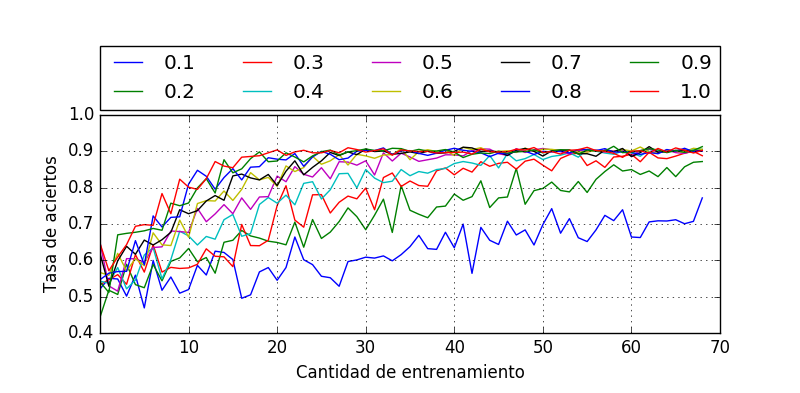
\includegraphics[width=\textwidth]{img/exp1.png}
\caption{Experimento con una hidden layer para distintos valores de learning rate} \label{img1}
\end{figure}

\begin{figure}[ht!]
\centering 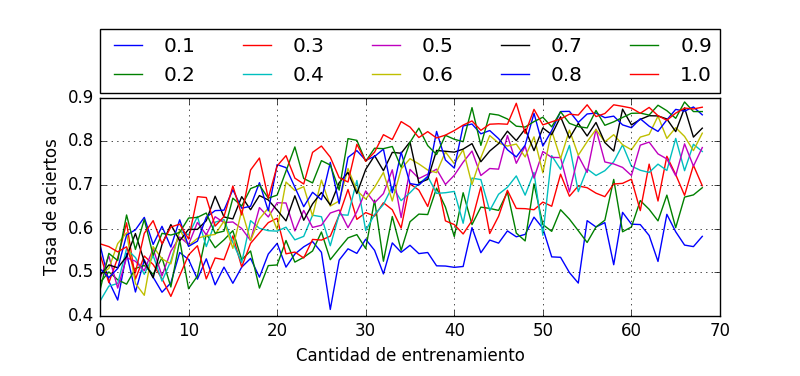
\includegraphics[width=\textwidth]{img/exp2.png}
\caption{Experimento con dos hidden layer para distintos valores de learning rate} \label{img2}
\end{figure}
\clearpage
\section{Análisis de Resultados}
Se observa de los resultados obtenidos que la red neuronal logró predecir de
mejor forma con más entrenamiento. El valor de 0.5 para pocos datos de entrenamiento
se esperaba, pues en esta fase la red neuronal se comporta de forma aleatoria.
Se observa una tasa de acierto que asciende hasta $0.9$ con el número de
entrenamientos adecuedo.\\

Se observa que una variación en la estructura de la red neuronal impacta en la
velocidad con que aprende la red. La red con dos hidden layers aprendió más lento
que la red con sólo un hidden layer. Esto se justifica en que la propagación del
error es más directa en el caso de menos layers, pero puede ser que esta construcción
tenga mayor sesgo y no funcione correctamente ante la presentación de una mayor cantidad
de casos de prueba.\\

Con respecto a la variación del learning rate, la velocidad de aprendizaje aumenta con
este. En el caso de la red neuronal con un hidden layer, se observa que la diferencia
entre learning rates mayores a 0.5 comienza a ser despreciable.\\

El experimento completo tomó 6 minutos en ejecutarse. Considerando
que este dataset era pequeño, se concluye que la red no es óptima en tiempo de ejecución, y que se podría
optimizar utilizando operaciones de matrices en vez de un enfoque orientado a objetos y
recursividad.

\section{Conclusión}
Se concluye que la red neuronal fue capaz de aprender sobre el problema de las
muestras de semen e infertilidad, logrando predecir hasta el 90\% de los casos
del set de pruebas.\\

Se concluye que el \textit{learning rate} y la cantidad de \textit{hidden layers}
impacta en la tasa de aprendizaje de la red.



% ============= FIN DE DOCUMENTO ==============
\end{document}

% % ················ IMAGEN ·················
% \begin{figure}[ht!]
% \centering
% \fbox{\includegraphics[scale=0.6]{img/flujo.png}}
% \caption{Flujo de caja anual}\label{flujo}
% \end{figure}
% %··········································

% % ················ IMAGEN DOBLE ·················
% \begin{figure}[ht!] \centering
% \subfloat[Esquemático]{\includegraphics[scale=0.44]{img/seguidor.png}}
% \subfloat[Simulación]{\includegraphics[scale=0.45]{img/seguidor1.png}}
% \caption{Simulación como seguidor de voltaje}\label{seguidor}
% \end{figure}
% %··········································
